\documentclass[10pt,a4paper,twoside,twocolumn,openany]{book}
% we'll need the old hline later
\let\oldhline\hline

\usepackage[bg-a4]{dnd} % Options: bg-a4, bg-letter, bg-full, bg-print, bg-none.
\usepackage{ifxetex}

\ifxetex
	\usepackage{fontspec}
\else
	\usepackage[francais]{babel}
	\usepackage[utf8]{inputenc}
\fi
\usepackage[most]{tcolorbox}
\usepackage{caption}

\begin{document}

\begin{tikzpicture}[remember picture,overlay]
\node[inner sep=0pt] (background) at (current page.center) {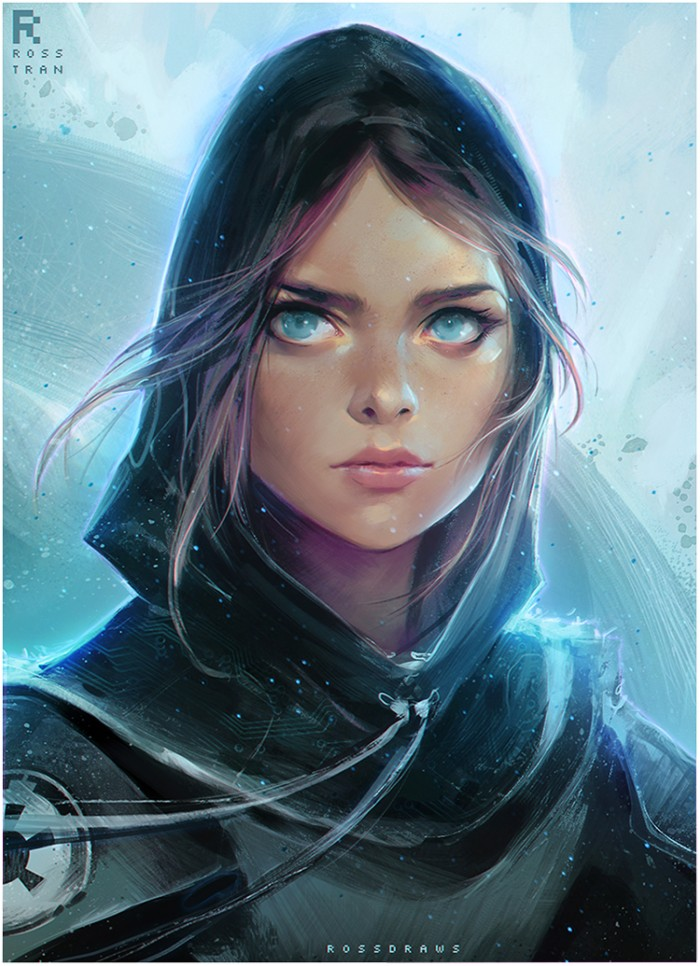
\includegraphics[width=\paperwidth,height=\paperheight]{lucy1.jpg}};
\draw (current page.center) node [fill=yellow!30!white,fill opacity=0.6,text opacity=1,inner sep=1cm]{\Huge\centering\bfseries\sffamily\parbox[c][][t]{\paperwidth}{\centering Lucy\\[15pt] % Book title
{\Large Le savoir est le seul trésor pour lequel plus on le partage, plus il grandit.}}};
\end{tikzpicture}

\chapter{Lucy}

\section{Description}

Je m'appelle Lucy Amastacia (Fleur d'étoile en commun), Je suis née en 1470.

Je suis relativement petite, je l'assume, 1m52. Cela m'a bien servi
pour l'instant. J'ai les cheveux brun, voir châtain sur le côté, légèrement
ondulés. J'ai les yeux bleus profonds, hérités à ce qu'on m'a dit de ma mère.
Je suis souvent habillée avec mes vêtement en cuir ; j'aime leur odeur, il m'arrive
même de dormir avec. Le cuir a travaillé et s'est adapté à ma morphologie.

Je porte souvent ma rapière rangée dans son fourreau, cela a le grand bénéfice d'éloigner
les agresseurs de pacotille. Je possède également 2 dagues, coincées
entre ma taille et ma ceinture, et enfin un petit couteau dont je me sers pour
découper ma nourriture, le pain est souvent raci et il faut bien un couteau pour le partager
avec mes compagnons du soir.

J'ai toujours avec moi Tchise, ma souris, elle m'a adoptée un soir de déprime. Je me cachais
depuis déjà 4 heures sous un trottoir de Lunargent et elle m'a tenu compagnie pendant
les 2 heures suivantes. Sans elle j'aurais perdu patience et je me serais probablement
fait prendre. Encore aujourd'hui quand je m'ennuie, je lui chantonne des notes, j'ai la
certitude qu'elle comprend ma musique. C'est notre manière de communiquer.

\begin{figure}[!h]
\centering
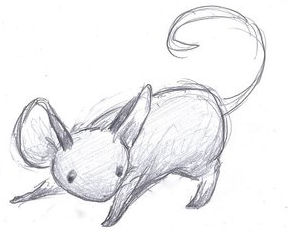
\includegraphics[scale=1]{tchise.png}
\caption*{Tchise, dessinée par Lucy}
\end{figure}

\begin{commentbox}{Lucy en quelques points}

\begin{itemize}
\item jolie et athlétique grâce à son ascendance elfe
\item méfiante envers l'autorité et les adultes
\item les pères sont des oppresseurs
\item curieuse et avide de savoir
\item elle pose trop de questions
\end{itemize}

\end{commentbox}

\section{Ma famille}

J'ai été élevée par une famille d'accueil jusqu'à l'age de 12 ans. Je hais ma famille.
Salomée, ma "mère" n'était pas une mauvaise personne, mais se soumettait trop
facilement a la volonté de mon beau père. Elle, me parlait parfois 
de ma vraie mère qui m'avait confiée à ses soins car sa vie d'aventurière était incompatible
avec la garde d'un enfant. Ma vraie mère est quelqu'un de bien mais elle a été trompée par mon
père adoptif. C'est un homme exécrable, je le déteste, je ne suis qu'un fardeau pour lui. Il 
m'a toujours considérée comme une moins que rien, un enfant bâtard illégitime. Il n'aime pas
les elfes, c'est pour lui une sous race.

Mes trois "soeurs" ne m'ont jamais acceptée, jalouses de ma beauté (j'ai surpris une
de leur conversation). A 12 ans j'avais déjà les formes et la prestance d'une jeune fille de 16
ans. Elle ne l'ont jamais supporté. J'étais pour elles une concurrence déloyale, alors que je n'ai
jamais demandé a être ce que je suis, je suis juste née comme cela.

Seul mon demi petit frère, poussin comme je l'appelais, venait se blottir dans me bras
les nuits ou je sanglotais. Il était la seule raison pour laquelle je suis resté dans cette famille,
je voulais le protéger, de ses soeurs et de son crétin de père.

A l'âge de 13 ans, j'ai décidé de fuir le foyer, et me suis intégrée dans un squat, au sud ouest de la ville
prêt du conservatoire de musique d'Utrumn.
Régulièrement, j'allais observer l'entrée et la sortie des musiciens, en imaginant à quoi pouvait ressembler
un concert. 

Au sein du squat j'ai pu rencontrer une foultitude de gens plus ou moins fréquentables, ils m'ont appris
à survivre par moi-même dans cette ville. J'y ai appris la camaraderie, ou comment gagner le confiance de quelqu'un
et qu'on l'on est pas forcement seul face a l'oppression des puissants.


\section{Lunargent}

Je suis née a Lunargent, c'est ma ville, je la connais comme ma poche. Je la préfère la nuit, lorsque
les lumières artificielles se reflètent à la surface de la rivière, dansent alors des milliers de petits feux follets. 
J'aime m'assoir sur la berge les pieds dans l'eau après une nuit de travail, j'observe alors la soleil
se lever et faire disparaître les feux follets. Il est alors temps pour moi d'aller m'endormir.

\vspace{2cm}

\chapter{Chroniques Partie 1}

\backgroundsetup{
scale=1,
angle=0,
opacity=1,
contents={
		\ifodd\value{page}
			\includegraphics[width=\paperwidth]{\oddbackgroundimg}
			\else
			\includegraphics[width=\paperwidth]{\evenbackgroundimg}
		\fi
		}
}

\begin{quotebox}
Lucy tient régulièrement un journal. Le début est sous forme d'illustration car elle ne sait pas écrire, elle 
apprendra par la suite a l'école à lire et écrire le commun.

Les premières années du journal contiennent principalement des illustrations de son beau père qui la frappe et parfois la caresse à des 
endroits impropre à une relation père fille.
\end{quotebox}

\section{Ce soir je pars}

J'ai décidé de partir, de quitter ce foyer minable. Je vais regretter poussin, mais 
il peut toujours compter sur moi et j'irai surveiller régulièrement qu'il va bien.

\section{Le Squat}

Ma première nuit s'est bien passée. Visiblement le travail pour une jeune fille
à l'air aussi innocent que moi ne manque pas et ils m'ont acceptée de suite. J'ai
hâte de commencer et me rendre utile

Voila une semaine que je suis au squat, pour l'instant tout se passe bien. Je me 
suis fait un ami, Malak, un jeune nain qui m'a appris a me servir d'un kit de crochetage.
On est parti faire une farce au refuge de chien abandonné à coté, on a crocheté une vingtaine
de cage et il fallait voir le gros Bob courir après les chiens, comme s'il avait une chance de
les rattraper, l'imbécile.

\section{Mallon}
Mallon est notre chef. C'est quelqu'un en qui j'ai confiance, si je fais bien mon travail, il me
récompense justement et avec lui je n'ai jamais eu l'impression d'être une "fille" ou "elfe" ou
"bâtard" ou "orphelin". Parfois je dois faire des travaux un peu douteux, je n'ai rien contre voler
l'administration, les puissants ou ceux qui m'ont fait du mal, mais parfois j'ai l'impression que l'on
détrousse des gens qui sont aussi opprimés par les politiques que nous.

\section{Les démanteleurs}

Ce soir je fais plus que jamais partie de la guilde. J'ai défendu le quartier contre le gang des
démanteleurs qui cherche à prendre le dessus sur notre business.
Nous avons réussi avec Malak, Eriel et le Bourru à isoler un membre du gang. C'est le Bourru
qui l'a fait chuter, je me suis assise sur son dos, j'avais son tronc entre mes cuisses j'ai posé 
la lame de ma dague sur sa glotte. 

Il implorait la vie sauve, Eriel a commencé a crier: "Fini-le, achève ce chien !". Je les ai regardé,
le Bourru a cautionné "Vas y, fais le !". Malak m'a fait un léger hochement de tête, en signe
d'approbation. Sans tourner la tête j'ai alors pressé la lame sur sa gorge le plus fort possible,
et je l'ai faite glisser. Une gerbe de sang chaud ma aspergé la joue gauche.

Malak m'attrape alors par l'épaule: "Vite, ne restons pas la !". Peu après on se réfugie dans notre planque.
Mon coeur bat à plein régime. Le Bourru tout excité, m'acclame et avec ses deux grosses mains il étale
tout le sang que j'avais sur le joue gauche partout sur mon visage, accompagnant son geste d'un rire gras. 

J'ai mal dormi ce jour la.

\section{Soir de fête}

Pour mon quinzième anniversaire, Malak et le Bourru m'ont organisé une petite fête. C'est la première fois
que je fête un anniversaire. On s'est bien amusé. Eloriel a apporté du fisstek, il a fait chauffé une 
sorte de poudre dans un récipient puis a disposé le résultat sur une plaque. Après quelques minutes
que le mélange refroidisse, j'ai inspiré une partie du mélange.

Wow...

J'ai fini par chanter des chansons qui se moquaient de Mallon, j'imitais le Bourru et parodiait
les défauts de Malak. On a tous cru à un moment que le bourru allait s'étouffer avec ses propres rires.
Puis on s'est tous endormi, les un sur les autres. Mon meilleur et seul anniversaire.

\begin{quotebox}
Le fisstek est une drogue dure, qui désinhibe l'utilisateur, le rend euphorique et crée une forte dépendance.
Les effets a long terme sont peu connus.
\end{quotebox}

\section{Demain je suis riche !}

Mallon m'a recrutée pour participer a un casse. Il nous a promis à tous une énorme coup. Il l'a bien 
préparé, je dois mémoriser trois pages d'instruction. J'ai hâte. Vivement demain.

\section{Une année au temple d'Oghma}

Voila presque quatre mois que je n'ai pas pu écrire dans mon journal. Je les ai
passés en prison, je viens tous juste de sortir et ils m'ont rendu mes possessions.
Évidemment ils ont confisqué le fisstek, je vais devoir m'en procurer au plus vite.
 
Les juges m'ont dit qu'ils avaient été cléments, en raison de mon jeune âge. Je dois servir un an
chez les prêtres d'Oghma, ou je méditerai mes méfaits. je devrai également reverser l'intégralité 
de mes gains durant cette année au garde que j'ai grièvement blessé et qui a faillit mourir.

Quelle poisse...

\section{Deux amis me rendent visite}

Aujourd'hui Malak est venu me rendre visite au Manoir de L'Inspiration.
Il avait Tchise avec lui. J'ai pleuré instantanément.
J'ai de suite inspecté ma souris, je connais Malak et il aurait pu tenter de remplacer Tchise par une autre
qui lui ressemblerait, s'il avait pensé que cela me ferait plaisir. 

Je vais à nouveau pouvoir chanter pour Tchise. J'étais tellement heureuse d'avoir revu
Malak que j'ai longuement embrassé ce roublard de nain sur la bouche lorsqu'il m'a dit au revoir. Je crois qu'il ne s'y 
attendait pas et moi non plus.

Il m'a glissé une dose de fisstek dans la poche. Je vais pouvoir planner ce soir, j'ai tellement hâte que la journée 
se finisse.

\section{L'année se termine}
Demain je finis mon année au temple d'Oghma. Je n'ai rencontré que des gens sincères ici.
J'ai pu apprendre énormément, ces gens ont une culture incroyable, ils ont mis à ma 
disposition des trésors de connaissances alors que je n'étais qu'un repris de justice.
Bien sur, j'ai du vivre sous quelques contraintes mais globalement je n'ai croisé
que des savants bienveillants.

J'ai pu apprendre à lire et écrire l'elfique, la langue de mon père, ainsi que le nain, que je parlais
déjà un peu avec Malak. Je suis sur que ça lui fera plaisir lorsque je lui passerai de petits morceaux
de papier sur lesquels je lui écrirai en nain ce que je pense de lui.

J'ai pu également apprendre la théorie de la musique, l'histoire de Lunargent, et quelques légendes
de Faerun.
J'ai surtout appris a quel point ma vie pourrait être différente de ce qu'elle a été
jusque la. On m'a proposé de devenir acolyte d'Oghma, je suis à la fois flattée, considérant
d'où je viens, mais un peu effrayée à l'idée de passer toute ma vie dans un temple.

Heureusement ils m'ont dit que j'avais tout mon temps pour considérer leur proposition, et que le
simple fait de prier Oghma, a vivre selon son dogme faisait de moi un serviteur 
d'Oghma. Certains de leur prêtres partent également a l'aventure répandre le savoir et la connaissance
dans des régions qui n'ont pas la chance d'avoir accès à ces trésors.

J'ai pour l'instant décliné la proposition, sans ressentiment.

\section{Enfin libre !}

La bibliothèque du manoir est incroyable, malgré tout je n'ai rien trouvé sur mes parents. 
La famille Cognedur n'était visiblement pas très renommée. Mais je ne désespère pas.

Je vais partir à l'aventure et retrouver la trace de mes parents. Je veux savoir exactement
ce qu'il s'est passé, s'ils sont encore vivants. Je ne retournerai donc pas au squat, j'écrirai
peut-être à Malak, je lui dois bien cela, mais je le ferai une fois sortie de cette ville car
Mallon ne verra probablement pas d'un bon oeil mon émancipation.

Je ne suis pas seule, Tchise est toujours avec moi.

\begin{quotebox}
Les informations connues de Lucy actuellement restent à définir.

Le père de Lucy, Soil Amastacia est un elfe de la lune originaire de Suzail.
La mère de Lucy, Amanda Duschène, est une humaine originaire de Sundabar.

Ses deux parents se sont rencontrés et aimés aux cours d'aventures.

Le grand père paternel est Raymond Duschène, humain originaire de Padhiver, 
la grand mère, Synelle Cognedur de son nom de jeune fille, est elle aussi
originaire de Padhiver.
\end{quotebox}

\chapter{Chroniques Partie 2}

A suivre...

\onecolumn
\chapter{Annexes}

\section{La Côte Des Epées} 

\begin{figure}[!h]
\centering
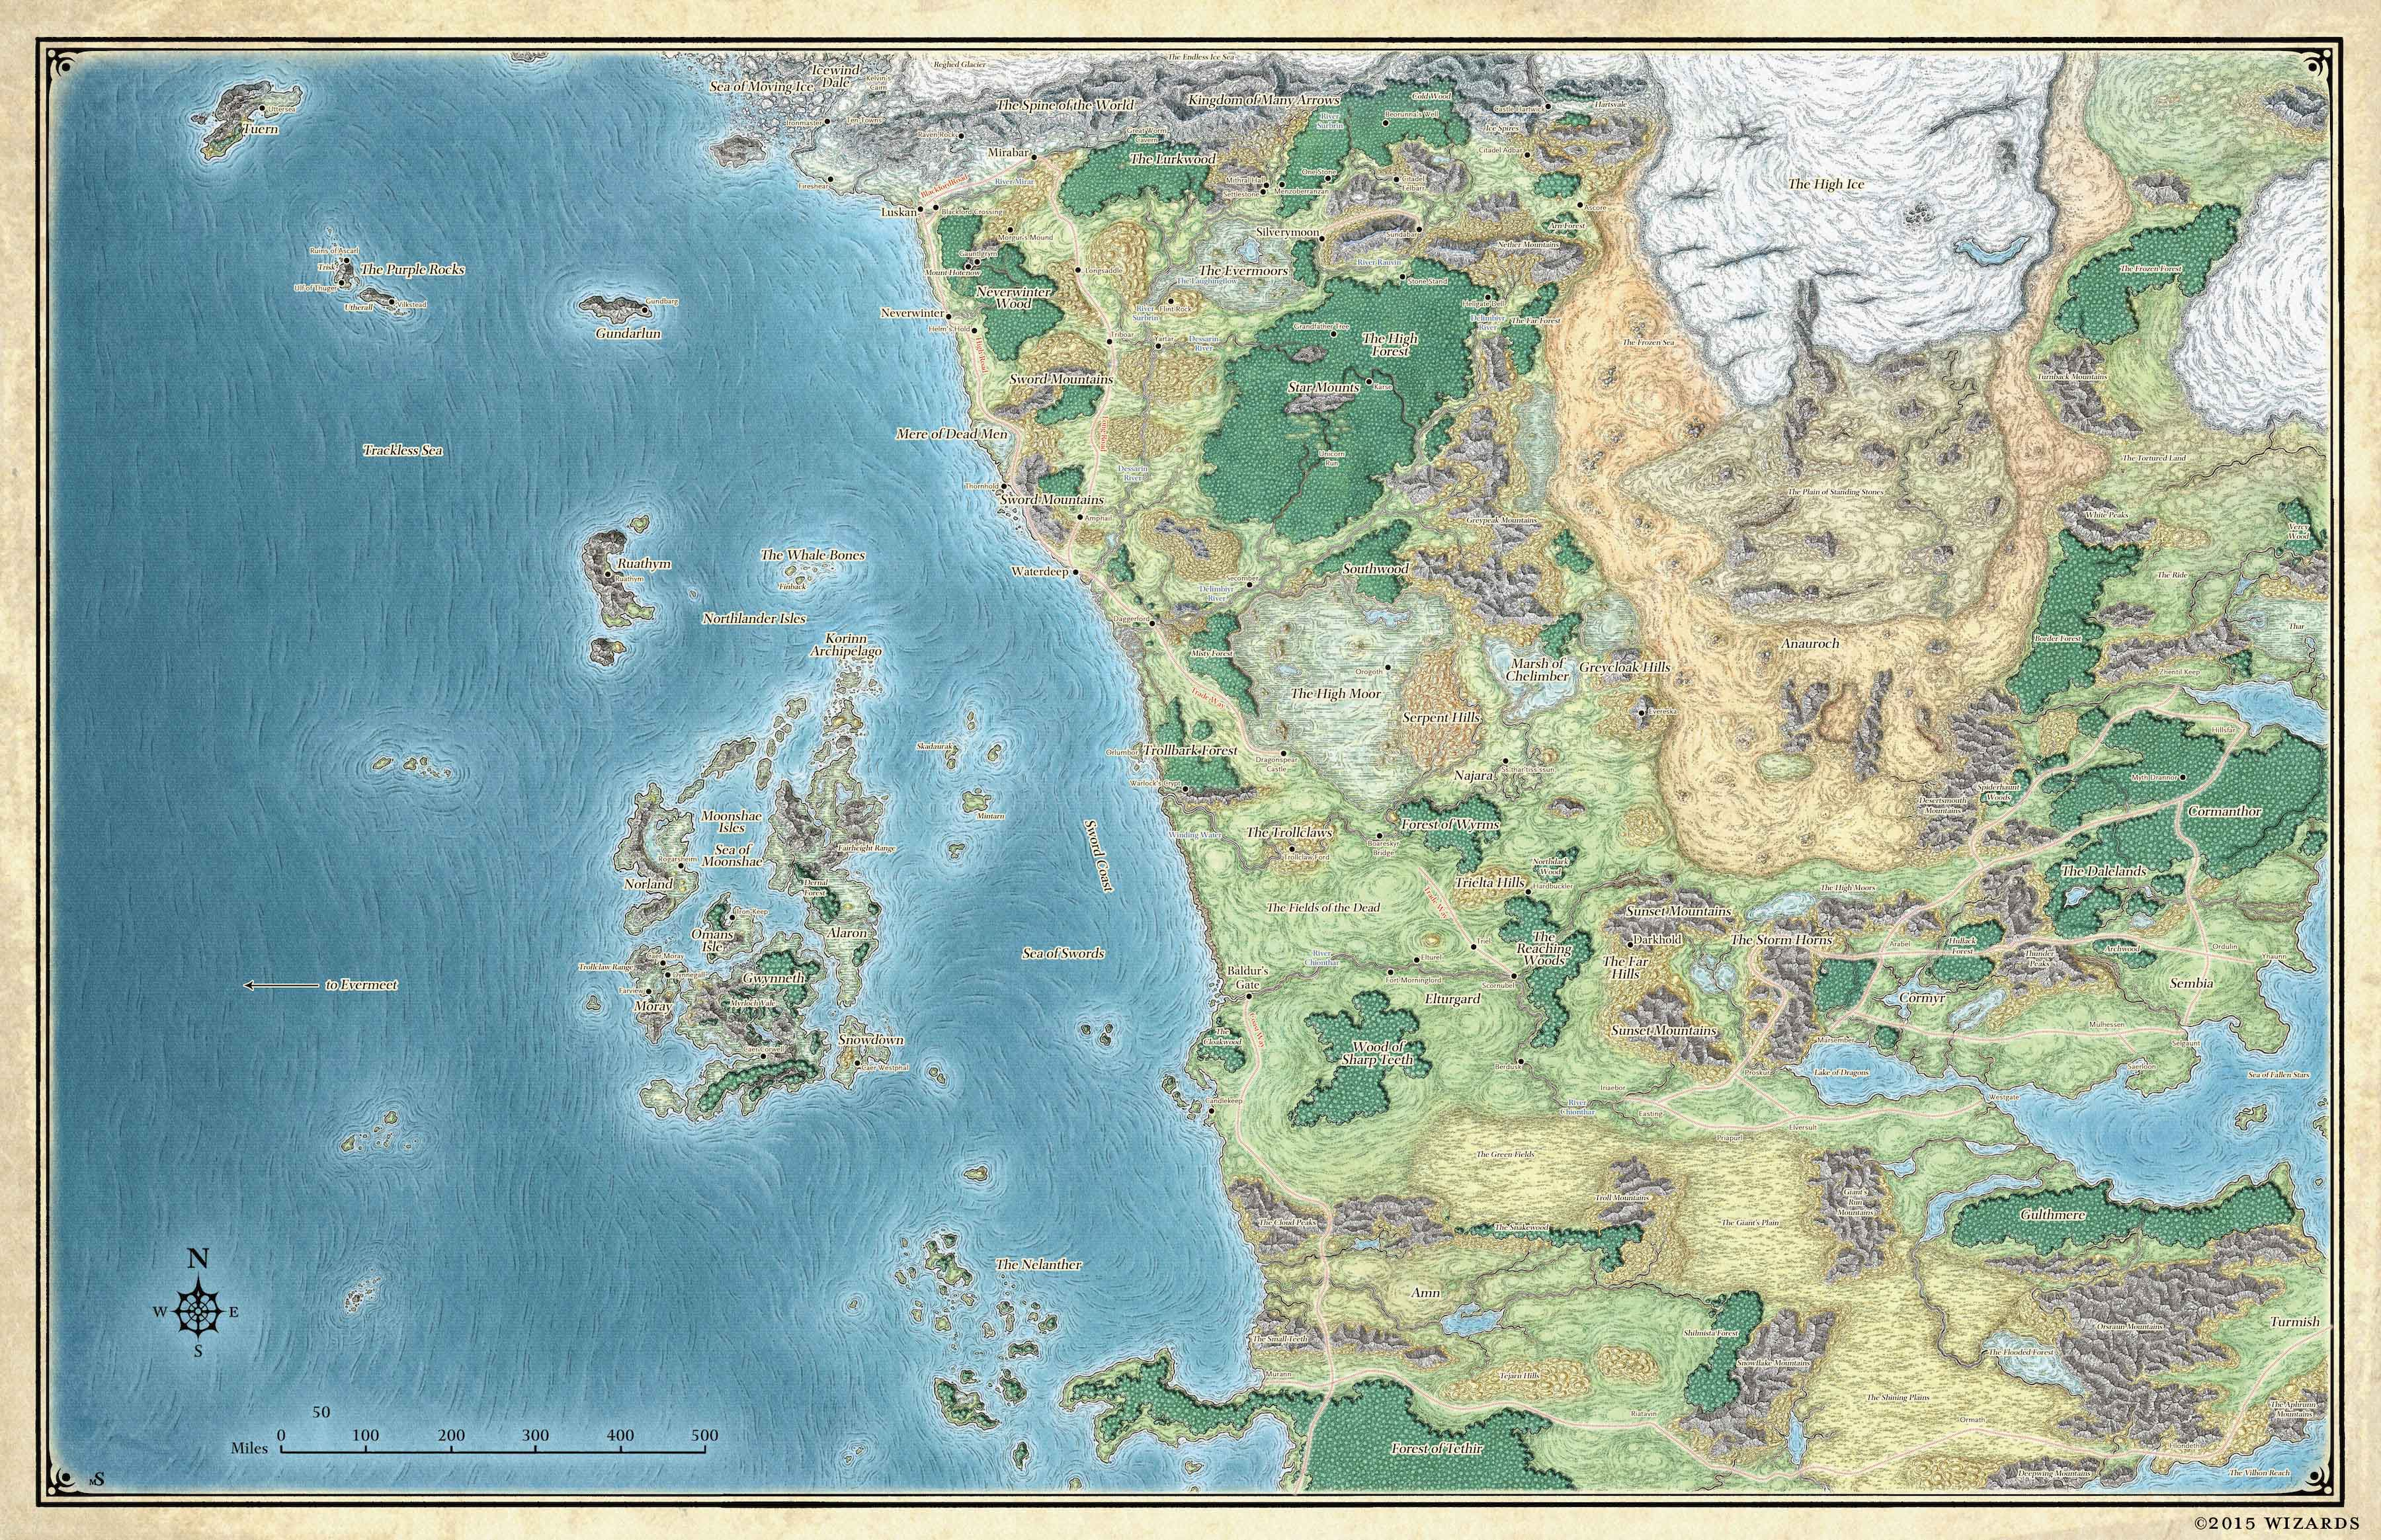
\includegraphics[width=\textwidth,keepaspectratio]{soc.jpg}
\end{figure}

\newpage

\section{Lunargent}

\begin{figure}[!h]
\centering
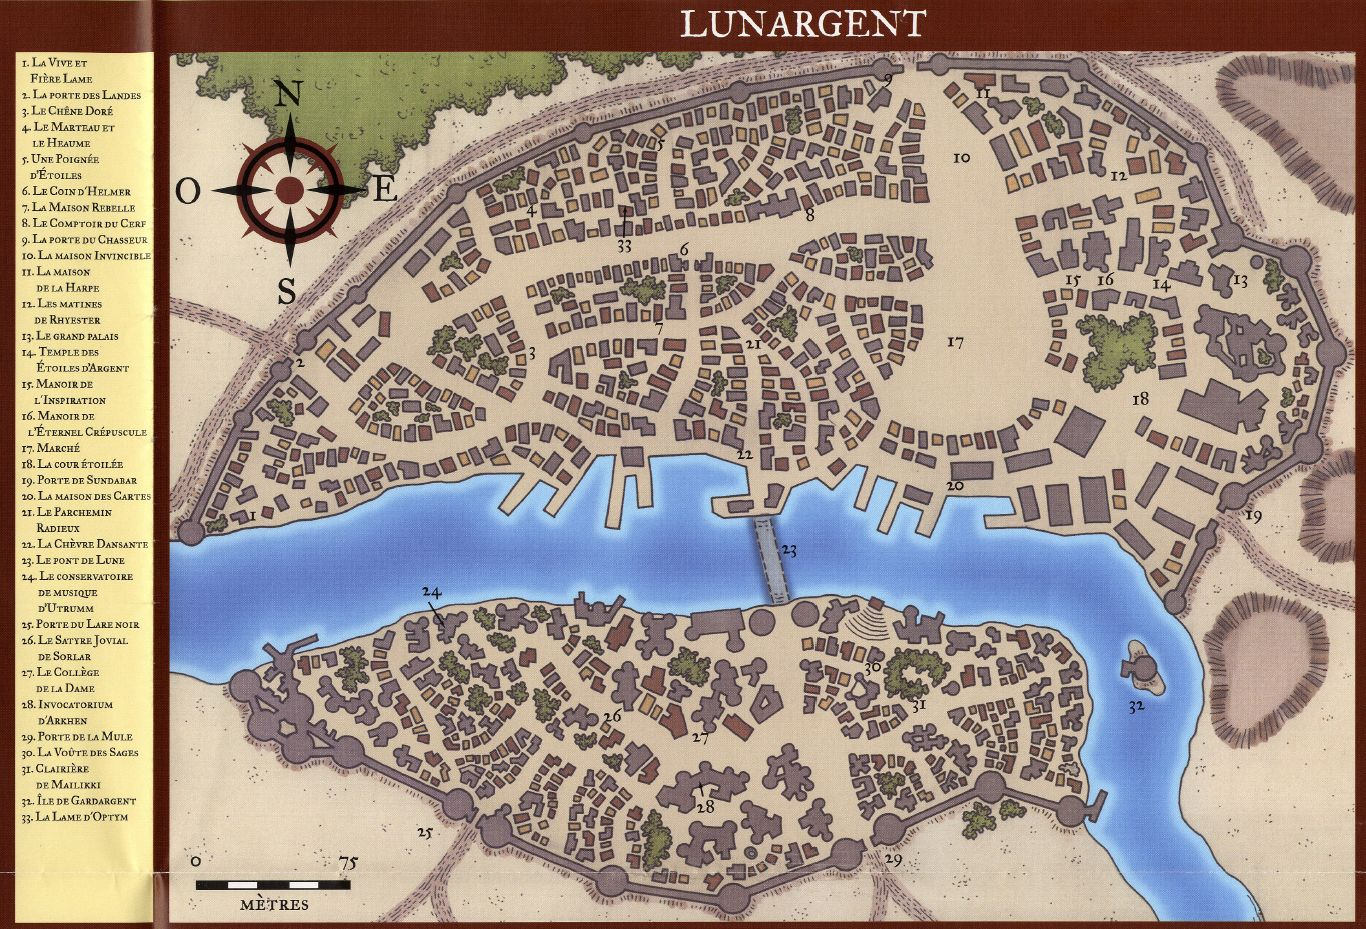
\includegraphics[width=\textwidth,keepaspectratio]{Map_Lunargent.jpg}
\end{figure}

\end{document}
